% ============================================================================
\section{Classical ASR}
% ============================================================================

\begin{frame}{Classical ASR: The Noisy Channel Model}
  \begin{itemize}
    \item \textbf{Search through space of all possible sentences.}
    \item \textbf{Pick the one that is most probable given the waveform.}
  \end{itemize}
  \begin{center}
    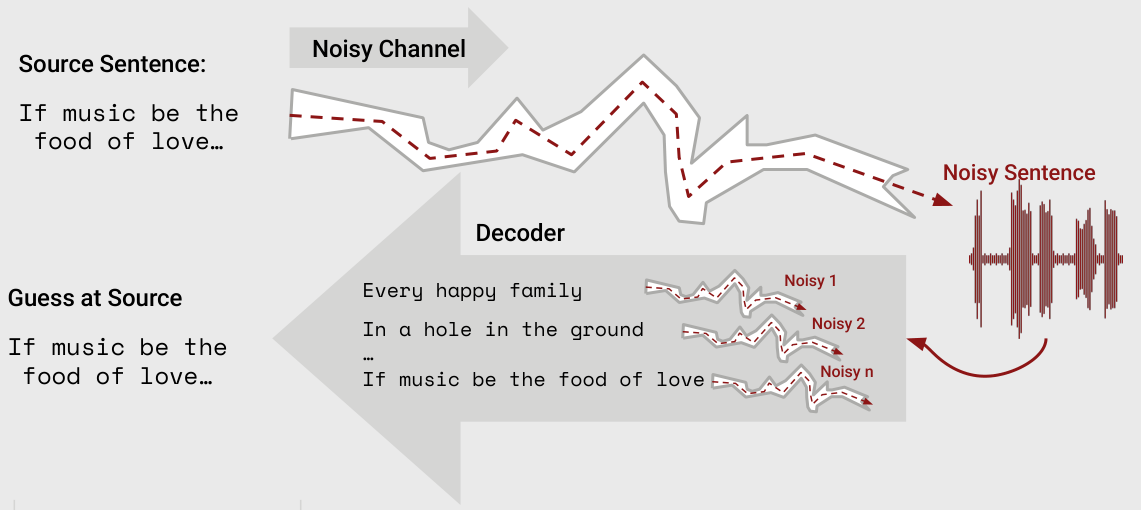
\includegraphics[width=\textwidth,height=0.70\textheight,keepaspectratio]{images/stt/stt_noisy_channel_model.png}
  \end{center}
  \slideimgsource{Stanford CS224S, Lecture 9 (2025 Spring), slide 5.}
\end{frame}

\begin{frame}{The Noisy Channel Model}
  \begin{itemize}
    \item What is the most likely sentence out of all sentences in the language $L$ that generated some given
    \textbf{acoustic input} $O$?
    \item Treat acoustic input $O$ as sequence of individual observations:
    \begin{itemize}
      \item[] $O = o_1, o_2, \ldots, o_T$
    \end{itemize}
    \item Define a sentence as a sequence of words:
    \begin{itemize}
      \item[] $W = w_1, w_2, \ldots, w_n$
    \end{itemize}
  \end{itemize}
  \vfill
\end{frame}

\begin{frame}{The Noisy Channel Model}
  \begin{itemize}
    \item \textbf{Probabilistic implication:} Pick the highest probability word sequence $W$:
      \begin{align*}
        \widehat{W} &= \arg\max\limits_{W \in L} P(W \mid O)
      \end{align*}
    \item \textbf{We can use Bayes' rule to rewrite this:}
      \begin{align*}
        \widehat{W} &= \arg\max\limits_{W \in L} \frac{P(O \mid W) P(W)}{P(O)}
      \end{align*}
    \item Since denominator is the same for each candidate sentence $W$, we can ignore it for the argmax:
      \begin{align*}
        \widehat{W} &= \arg\max\limits_{W \in L} P(O \mid W) P(W)
      \end{align*}
  \end{itemize}
  \vfill
\end{frame}

\begin{frame}{The Noisy Channel Model}
  \centering
  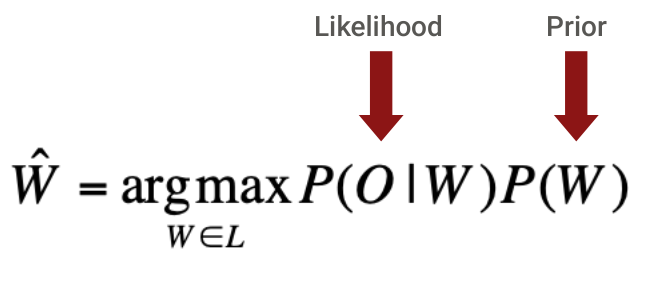
\includegraphics[width=\textwidth,height=0.84\textheight,keepaspectratio]{images/stt/stt_noisy_channel_equation.png}
  \slideimgsource{Stanford CS224S, Lecture 9 (2025 Spring), slide 9.}
\end{frame}

\begin{frame}{Word error rate (WER)}
\centering
  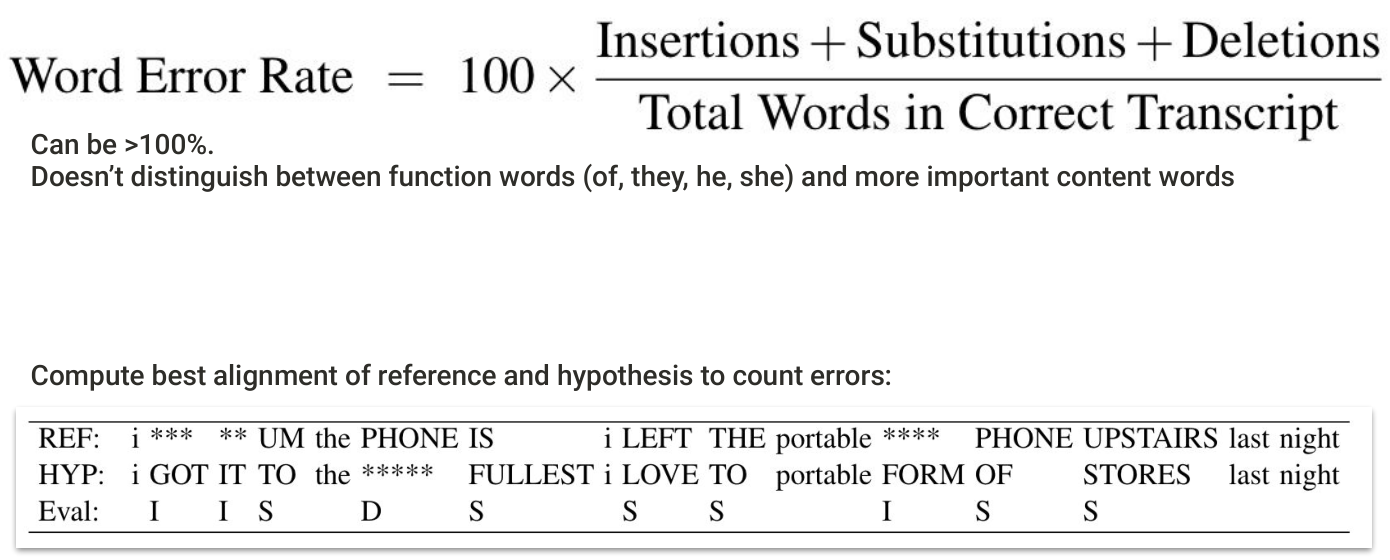
\includegraphics[width=\textwidth,height=0.80\textheight,keepaspectratio]{images/stt/stt_word_error_rate.png}
  \slideimgsource{Alignment example after Jurafsky \& Martin, \textit{Speech and Language Processing}; via Stanford CS224S, Lecture 9 (2025 Spring), slide 11.}
\end{frame}

\begin{frame}{Speech Recognition Architecture}
  \centering
  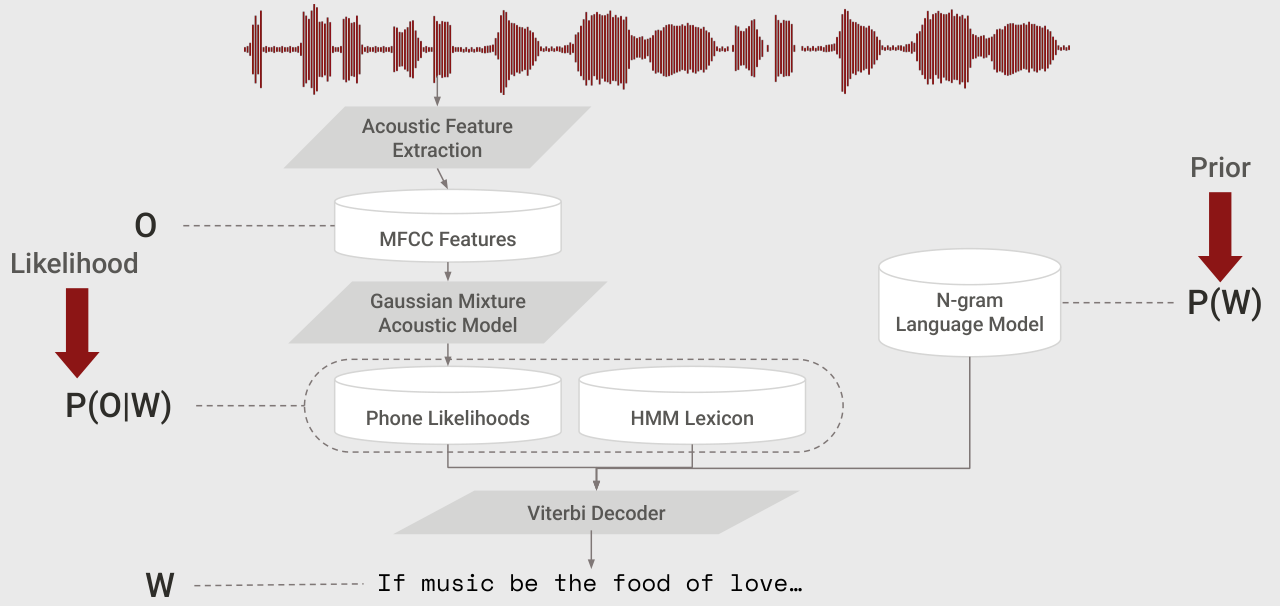
\includegraphics[width=\textwidth,height=0.84\textheight,keepaspectratio]{images/stt/stt_asr_architecture.png}
  \slideimgsource{Stanford CS224S, Lecture 9 (2025 Spring), slide 13.}
\end{frame}

\begin{frame}{Classical ASR: HMM-GMM system}
  \centering
  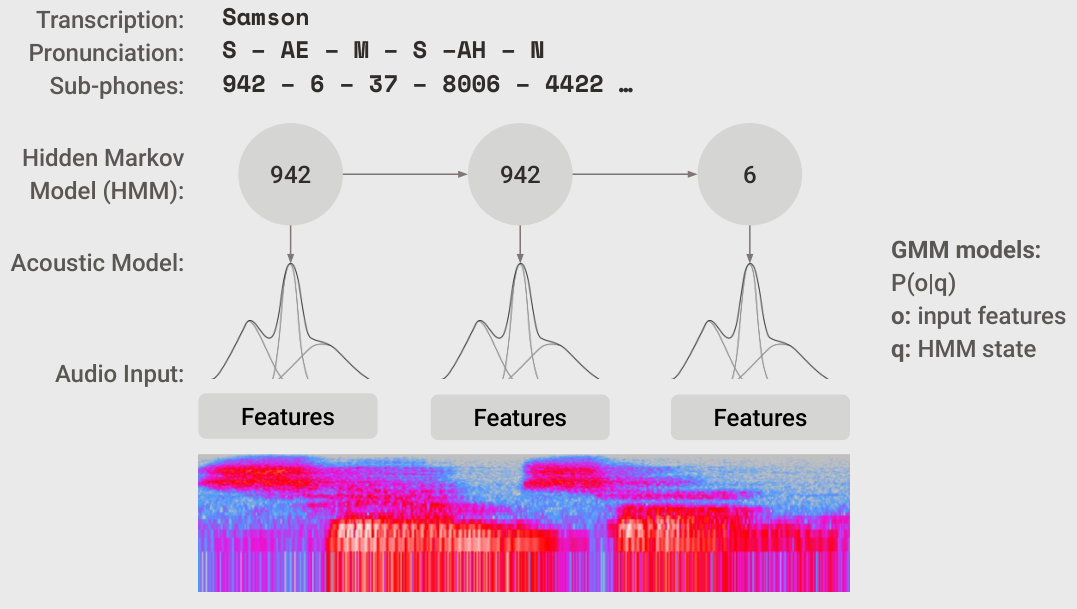
\includegraphics[width=\textwidth,height=0.84\textheight,keepaspectratio]{images/stt/stt_hmm_gmm_phones.png}
  \slideimgsource{Stanford CS224S, Lecture 9 (2025 Spring), slide 16.}
\end{frame}
